% NB: use pdflatex to compile NOT pdftex.  Also make sure youngtab is
% there...

% converting eps graphics to pdf with ps2pdf generates way too much
% whitespace in the resulting pdf, so crop with pdfcrop
% cf. http://www.cora.nwra.com/~stockwel/rgspages/pdftips/pdftips.shtml




\documentclass[10pt,aspectratio=169,dvipsnames]{beamer}
\usetheme[color/block=transparent]{metropolis}

\usepackage[absolute,overlay]{textpos}
\usepackage{booktabs}
\usepackage[utf8]{inputenc}


\usepackage[scale=2]{ccicons}

\usepackage[official]{eurosym}

%use this to add space between rows
\newcommand{\ra}[1]{\renewcommand{\arraystretch}{#1}}


\setbeamerfont{alerted text}{series=\bfseries}
\setbeamercolor{alerted text}{fg=Mahogany}
\setbeamercolor{background canvas}{bg=white}


\newcommand{\R}{\mathbb{R}}

\def\l{\lambda}
\def\m{\mu}
\def\d{\partial}
\def\cL{\mathcal{L}}
\def\co2{CO${}_2$}



% for sources http://tex.stackexchange.com/questions/48473/best-way-to-give-sources-of-images-used-in-a-beamer-presentation

\setbeamercolor{framesource}{fg=gray}
\setbeamerfont{framesource}{size=\tiny}


\newcommand{\source}[1]{\begin{textblock*}{5cm}(10.5cm,8.35cm)
    \begin{beamercolorbox}[ht=0.5cm,right]{framesource}
        \usebeamerfont{framesource}\usebeamercolor[fg]{framesource} Source: {#1}
    \end{beamercolorbox}
\end{textblock*}}

\usepackage{hyperref}


%\usepackage[pdftex]{graphicx}


\graphicspath{{graphics/}}

\DeclareGraphicsExtensions{.pdf,.jpeg,.png,.jpg}



\def\goat#1{{\scriptsize\color{green}{[#1]}}}



\let\olditem\item
\renewcommand{\item}{%
\olditem\vspace{5pt}}

\title{Energy System Modelling\\ Summer Semester 2019, Lecture 1}
%\subtitle{---}
\author{
  {\bf Dr. Tom Brown}, \href{mailto:tom.brown@kit.edu}{tom.brown@kit.edu}, \url{https://nworbmot.org/}\\
  \emph{Karlsruhe Institute of Technology (KIT), Institute for Automation and Applied Informatics (IAI)}
}

\date{\vspace{.3cm}6th June 2019}


\titlegraphic{%
  \vspace{6cm}
  \hspace{10cm}
    \includegraphics[trim=0 0cm 0 0cm,height=1.8cm,clip=true]{kit.png}
}

\begin{document}

\maketitle


\begin{frame}

  \frametitle{Table of Contents}
  \setbeamertemplate{section in toc}[sections numbered]
  \tableofcontents[hideallsubsections]
\end{frame}


\section{Administration}




\begin{frame}
  \frametitle{Contact Details}

  Dr. Tom Brown

  Young Investigator Group Leader

  Energy System Modelling Research Group

  Institute for Automation and Applied Informatics (IAI)

  KIT, North Campus

  \href{mailto:tom.brown@kit.edu}{tom.brown@kit.edu}

  Group website (with \alert{open MA theses}): \url{https://www.iai.kit.edu/english/ESM.php}

  Personal website: \url{https://nworbmot.org/}

I am a physicist who has specialised in the optimisation of energy
systems and the interactions of complex networks. I now work at the
intersection of informatics, economics, engineering, mathematics,
meteorology and physics.

\end{frame}



\begin{frame}
  \frametitle{Lectures and Exercise Classes}

  \alert{Dates:} Thu 6.6, Fri 7.6, Thu 13.6, Fri 14.6, Thu 27.6

  Each day will consist of 3 lectures and one exercise class:

  \vspace{.2cm}

  \centering
  \begin{tabular}{@{} p{3cm}p{6cm} @{}}

  09:00-10:30 & Lecture 1 \\
  10:45-12:15 & Lecture 2 \\
  13:00-14:30 & Exercise Class \\
  14:45-16:15 & Lecture 3 \\
\end{tabular}

  \vspace{.2cm}
  \raggedright

  Some of the exercises will require you to program in Python, so
  please bring a laptop. We will help you to install Python and the
  requisite libraries.

  \vspace{.2cm}

  The course has 4 ECTS points.

  \vspace{.2cm}



  \alert{Location:} Campus Nord, Building 449, Room 126



\end{frame}


\begin{frame}
  \frametitle{Course Website}

  You can find the course website here:

  \url{https://nworbmot.org/courses/esm-2019/}

  by following the links from:

  \url{https://nworbmot.org/}

  Course notes, exercise sheets and other links can be found there.

\end{frame}




\begin{frame}
  \frametitle{Registration for Oral Exam}

  To get an evaluation at the end of the course, you need to register
  online for the oral examination.

  The oral examinations will take place some time in July on a
  single date. The date will be decided during the final lecture,
  based on when we are all available.

\end{frame}


\begin{frame}
  \frametitle{MA Theses}

  We have some exciting opportunities in the Energy System Modelling
  group at IAI to do MA Theses, see the list here:

  \url{https://www.iai.kit.edu/english/2552.php}

  We are also open to new suggestions and themes if they fit with our
  research programme.

\end{frame}

\begin{frame}
  \frametitle{Literature}

  There is no book which covers all aspects of this course. In particular there is no good source for the combination of data analysis, complex network theory, optimisation and energy systems. But there are lots of online lecture notes. The world of renewables also changes fast...

  The following are concise:
  \begin{itemize}
    \item Volker Quashning, ``Regenerative Energiesysteme'', Carl Hanser Verlag München, 2015
      \item      Leon Freris, David Infield, ``Renewable Energy in Power Systems'', Wiley, 2006
      \item Göran Andersson Skript, ``Elektrische Energiesysteme: Vorlesungsteil Energieübertragung,'' online
          \item D.R.~Biggar, M.R.~Hesamzadeh, ``The Economics of Electricity
  Markets,'' Wiley, 2014
  \end{itemize}

\end{frame}




\section{Course outline}


\begin{frame}
  \frametitle{What is Energy System Modelling?}

  \alert{Energy System Modelling} is about the overall \alert{design} and \alert{operation} of the energy system.

  How can we fulfil energy policy targets
  of \alert{sustainability}, \alert{reliability} and
  \alert{affordability}?

\vspace{1cm}
  \centering
    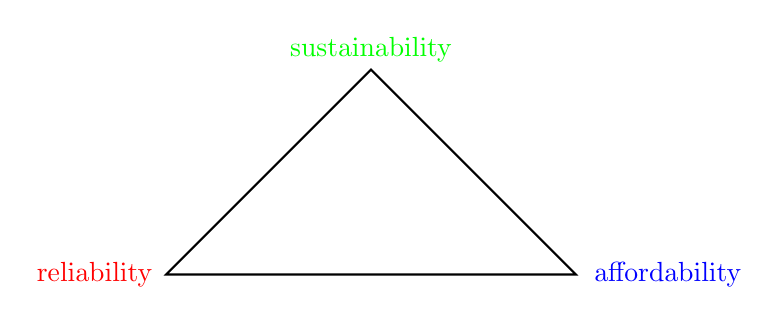
\begin{tikzpicture}[thick,scale=1.3]

      \coordinate (O) at (0,0);
      \coordinate (A) at (4,0);
      \coordinate (B) at (2,2);
      \draw (O)--(A)--(B)--cycle;
      \draw (2,2.2) node[green]{sustainability};
      \draw (-0.7,0) node[red]{reliability};
      \draw (4.9,0) node[blue]{affordability};
  \end{tikzpicture}


\end{frame}

\begin{frame}
  \frametitle{What is Energy System Modelling?}

  \begin{itemize}
  \item \alert{Sustainability}: Can we supply energy while respecting environmental constraints (greenhouse gas emissions, preservation of wildlife), as well as social and political constraints (public acceptance of transmission lines, onshore wind, nuclear power, etc.)?
  \item \alert{Reliability}: Can we ensure energy services are delivered whenever needed, even when the wind isn't blowing and the sun isn't shining, and even when components fail?
  \item \alert{Affordability}: Can we deliver energy at a reasonable cost?
  \end{itemize}

  \vspace{1cm}

  Some of these policy targets can come into \alert{conflict} $\implies$ \alert{energy trilemma}.


\end{frame}


\begin{frame}
  \frametitle{Course outline}

  This course will cover the following topics:

  \begin{itemize}
  \item General properties of renewable power, time series analysis
    \item Backup generation, curtailment
  \item Network modelling in power systems
  \item Storage modelling
  \item Optimization theory
  \item Energy system economics
    \item Dynamics of renewable energy networks (synchronization, etc.)
      \item Complex network techniques for renewable energy networks (flow tracing, etc.)
  \end{itemize}


\end{frame}






\section{The Greenhouse Gas Challenge}


\begin{frame}
  \frametitle{2015 Paris Agreement}

  The 2015 Paris Agreement pledged its signatories to
 `pursue efforts to limit [global warming above pre-industrial levels] to \alert{$1.5^\circ$C}' and
   hold `the increase...to \alert{well below $2^\circ$C}'.
  These targets were chosen to avoid potentially irreversible \alert{tipping points} in the Earth's systems.


  \begin{columns}[T]
\begin{column}{9.5cm}

  \includegraphics[width=10cm]{nclimate3013-f1.jpg}
\end{column}
\begin{column}{4.5cm}

  \vspace{.3cm}

  WAIS: West Antarctic Ice Sheet (5m sea level rise)

  \vspace{.2cm}

  Greenland (7m)

  \vspace{.2cm}

  THC: thermohaline circulation (warms Europe)

  \vspace{.2cm}

  ENSO: El Niño–Southern Oscillation (extreme weather)

  \vspace{.2cm}

  EAIS: East Antarctic Ice Sheet ($>50$ m)

\end{column}
  \end{columns}

\source{\href{https://www.nature.com/articles/nclimate3013}{`Why the right climate target was agreed in Paris'}, Nature Climate Change, 2016}
\end{frame}


\begin{frame}
  \frametitle{The Global Carbon Dioxide Challenge: Net-Zero Emissions by 2050}

  \begin{columns}[T]
\begin{column}{7.5cm}

  \includegraphics[width=8cm]{ipcc-sr15}


\end{column}
\begin{column}{6cm}
  \begin{itemize}
\item Scenarios for global CO$_2$ emissions that limit warming to 1.5$^\circ$C about industrial levels (\alert{Paris agreement})
\item Today emissions \alert{still rising}
\item Level of use of negative emission technologies (NET) depends on rate of progress
\item 2$^\circ$C target without NET also needs
  rapid fall by 2050
\item Common theme: \alert{net-zero by 2050}
\end{itemize}
\end{column}
  \end{columns}

    \source{\href{http://ipcc.ch/report/sr15/}{IPCC SR15 on 1.5C, 2018}}
\end{frame}

\begin{frame}
  \frametitle{The Greenhouse Gas Challenge: Net-Zero Emissions by 2050}

  Paris-compliant 1.5$^\circ$~C scenarios from European Commission - \alert{net-zero GHG in EU by 2050}

  \vspace{.4cm}

  %Figure 6 from https://ec.europa.eu/clima/sites/clima/files/docs/pages/com_2018_733_en.pdf
  \includegraphics[width=14cm]{eu-lts-net-zero.png}


    \source{\href{https://ec.europa.eu/clima/sites/clima/files/docs/pages/com_2018_733_en.pdf}{European Commission `Clean Planet for All', 2018}}
\end{frame}


\begin{frame}
  \frametitle{It's not just about electricity demand...}

  %GHG in 2016 are 4.291~Gt, CO2 is 3.489 ~Gt without LULUCF and without indirect
  %Global is 36.2 Gt (EU figure from carbonbrief excludes LULUCF, so assume global also)
%https://www.carbonbrief.org/analysis-global-co2-emissions-set-to-rise-2-percent-in-2017-following-three-year-plateau
  EU28 \co2{} emissions in 2016 (total 3.5~Gt \co2, 9.7\% of global):

  \centering
    % left bottom right top
  \includegraphics[trim=0 0.7cm 0 0.5cm,width=12cm]{EU28-emissions_pie-2016-CO2-190311.pdf}

%  ...\alert{but} wind and solar will dominate primary energy in all sectors, so electrification is critical.

  \source{Brown, data from \href{https://www.eea.europa.eu/data-and-maps/data/national-emissions-reported-to-the-unfccc-and-to-the-eu-greenhouse-gas-monitoring-mechanism-13}{EEA}}
\end{frame}



\begin{frame}
  \frametitle{...but electrification of other sectors is critical for decarbonisation}

\alert{Electrification is essential} to decarbonise sectors such as
transport, heating and industry, since we can use low-emission
electricity from e.g. wind and solar to displace fossil-fuelled
transport with electric vehicles, and fossil-fuelled heating with
electric heat pumps.

Some scenarios show a \alert{doubling or more of electricity demand}.

  \vspace{.7cm}

  \begin{columns}[T]
\begin{column}{6cm}
  \includegraphics[trim=0 0cm 0 0cm,width=6cm,clip=true]{tesla.jpg}
\end{column}
\begin{column}{6cm}

  \includegraphics[trim=0 0cm 0 0cm,width=6cm,clip=true]{640px-Heat_Pump.jpg}
\end{column}
\end{columns}



\source{Tesla; heat pump: \href{https://commons.wikimedia.org/w/index.php?curid=10795550}{Kristoferb at English Wikipedia}}

\end{frame}





\begin{frame}{Efficiency of renewables and sector coupling}


  \includegraphics[width=\linewidth,trim=2.7cm 20cm 3.2cm 1.8cm,clip=true]{./graphics/bmwi-whitepaper-figure_18.pdf}

  \source{\href{https://www.bmwi.de/Redaktion/EN/Publikationen/whitepaper-electricity-market.html}{BMWi White Paper 2015}}
\end{frame}



\begin{frame}[fragile]
  \frametitle{Why focus on wind and solar for electricity generation?}
    \begin{columns}[T]
      \begin{column}{4cm}
        \begin{itemize}
        \item construction and operation have low greenhouse gas emissions
        \item good wind and sun are available in many parts of the world
        \item worldwide potential that exceeds demand by many factors
        \item rapidly falling costs
        \end{itemize}
      \end{column}
      \begin{column}{5cm}
        \includegraphics[trim=0 0cm 0 0cm,width=4.5cm,clip=true]{SolarGIS-Solar-map-Germany-de}
      \end{column}
      \begin{column}{5cm}
        \vspace{.8cm}
        \includegraphics[trim=0 0cm 0 0cm,width=5.5cm,clip=true]{43_Mittlere_Windgeschwindigkeit_100_m_Deutschland}
      \end{column}
    \end{columns}


\end{frame}



\begin{frame}{Worldwide potentials}


    \begin{columns}[T]
      \begin{column}{8.5cm}
  \centering
    \includegraphics[width=8.7cm]{global_potentials.png}

      \end{column}
      \begin{column}{6cm}

    \vspace{.5cm}
        \begin{itemize}
        \item Potentials for wind and solar exceed current demand by many factors (ignoring variability)
        \item Other renewable sources include wave, tidal, geothermal, biomass and hydroelectricity
        \item Uranium depends on the reactor: conventional thermal reactors can extract 50-70 times less than fast breeders
        \end{itemize}
      \end{column}
    \end{columns}

      \source{\href{http://solarmarketpathways.org/wp-content/uploads/2017/08/NSC-Achieving-High-PV-Penetration-160526.pdf}{Perez et al, Applied Policy, 2016}}

\end{frame}

\begin{frame}{Low cost of wind \& solar per MWh in 2017 (NB: ignores variability)}

  LCOE = \alert{Levelised Cost of Energy} = Total Costs $/$ Energy Output
  \centering
  \includegraphics[width=14cm]{lazard-cropped.jpg}

  \source{\href{https://www.lazard.com/perspective/levelized-cost-of-energy-2017/}{Lazard's LCOE Analysis V11}}

\end{frame}







\begin{frame}[fragile]
  \frametitle{Must take account of variabilility \& social \& political constraints}



\begin{columns}[T]

  \begin{column}{5cm}


\centering
\includegraphics[width=5cm]{nein_zur_monstertrasse}

  \end{column}


  \begin{column}{6.7cm}

    \vspace{.5cm}

    Sustainability doesn't just mean taking account of environmental constraints.

    \vspace{.5cm}

    There are also \alert{social and political constraints},
    particularly for transmission grid and onshore wind
    development.

    \vspace{.5cm}

\includegraphics[width=7cm]{Protestplakat-gegen-den-Bau-von-Windraedern-in-Hamburg-Deutschland.jpg}

  \end{column}

\end{columns}

\end{frame}


\begin{frame}
  \frametitle{Energy Transition: Several changes happening simultaneously}

  \alert{Energiewende}: The Energy Transition, consists of several parts:

  \begin{itemize}
  \item Transition to an energy system with low greenhouse gas emissions
  \item Renewables replace fossil-fuelled generation (and nuclear in some countries)
  \item Increasing integration of international electricity markets
  \item Better integration of transmission constraints in electricity markets
  \item Sector coupling: heating, transport and industry electrify
  \item More decentralised location and ownership in the power sector
  \end{itemize}

\end{frame}


\begin{frame}
  \frametitle{Electricity generation in Germany per year}

  In 15 years Germany has gone from a system dominated by nuclear and
  fossil fuels, to one with 33\% renewables in electricity consumption.

  \centering
  \includegraphics[width=11cm]{germany_yearly_electricity}

  \source{Author's own representation based on \url{https://www.energy-charts.de/energy_en.htm}}
\end{frame}




\begin{frame}[fragile]
  \frametitle{What can informatics contribute?}

  In all these questions we are limited by \alert{computational complexity}.

  Informatics can contribute on the \alert{data side}:
  \begin{itemize}
  \item Processing and analysing enormous weather datasets
  \item Geographical potential analysis with GIS tools
  \item Visualisation of results
  \end{itemize}
  and on the \alert{algorithmic side}:
  \begin{itemize}
  \item Data reduction: clustering and PCA examples to follow later
  \item New optimisation routines for speed and accuracy
  \item Information theory to trace interdependencies
  \end{itemize}

  Build on informatics' \alert{interdisciplinary} links to engineering, economics, meteorology, mathematics and physics.
\end{frame}




\section{Introduction: Balancing Variable Renewable Energy in Europe}



\begin{frame}[fragile]
  \frametitle{Goals for Energy System Modelling}

  \begin{enumerate}
  \item What \alert{infrastructure} (wind, solar, hydro generators,
    heating/cooling units, storage and networks) does a highly renewable energy system
    require and \alert{where} should it go?
  \item Given a desired \co2 emissions reduction (e.g. 95\% compared to 1990),
    what is the \alert{cost-optimal} combination of infrastructure?
  \item How do we deal with the \alert{variablility} of wind and solar: balancing in space with networks or in time with storage?
  \end{enumerate}



\end{frame}


\begin{frame}
  \frametitle{Variability: Single wind site in Berlin}

  Looking at the wind output of a single wind plant over two weeks, it is highly
  variable, frequently dropping close to zero and fluctuating strongly.

  \centering
  \includegraphics[width=12cm]{variability-berlin}


\end{frame}



\begin{frame}
  \frametitle{Electricity consumption is much more regular}

  Electrical demand is much more regular over time - dealing with the
  \alert{mismatch} between locally-produced wind and the demand would
  require a lot of storage...

  \centering
  \includegraphics[width=12cm]{DE-load}


\end{frame}



\begin{frame}
  \frametitle{Variability: Different wind conditions over Germany}

  The wind does not blow the same at every site at every time: at a given time there are a variety of wind conditions across Germany. These differences \alert{balance out over time and space}.

  \centering
  \includegraphics[width=10cm]{2015-05-13-1100}

  \source{\url{https://earth.nullschool.net/}}

\end{frame}




\begin{frame}
  \frametitle{Variability: Single country: Germany}

  For a whole country like Germany this results in valleys and peaks that are  somewhat smoother, but the profile still frequently
  drops close to zero.

  \centering
  \includegraphics[width=12cm]{variability-de}


\end{frame}



\begin{frame}
  \frametitle{Variability: Different wind conditions over Europe}

  The scale of the weather systems are bigger than countries, so to leverage the full smoothing effects, you need to integrate wind at the \alert{continental scale}.

  \centering
  \includegraphics[width=10cm]{2015-11-30-0300}

  \source{\url{https://earth.nullschool.net/}}

\end{frame}



\begin{frame}
  \frametitle{Variability: A continent: Europe}


  If we can integrate the feed-in of wind turbines across the European continent, the
  feed-in is considerably smoother: we've eliminated most valleys and
  peaks.

  \centering
  \includegraphics[width=12cm]{variability-eu}


\end{frame}





\begin{frame}
  \frametitle{Variability: A continent: Wind plus Hydro}

  Flexible, renewable hydroelectricity from storage dams in Scandinavia and the Alps can fill many of the valleys; excess energy can either be curtailed (spilled) or stored.

  \centering
  \includegraphics[width=12cm]{variability-load}


\end{frame}



\begin{frame}
  \frametitle{Daily variations: challenges and solutions}

  \begin{columns}[T]
    \begin{column}{5cm}
      \includegraphics[trim=0 0cm 0 0cm,width=5cm,clip=true]{DE-solar-day.pdf}

      \includegraphics[trim=0 0cm 0 0cm,width=5cm,clip=true]{DE-transport-day.pdf}
    \end{column}
    \begin{column}{4cm}
      \alert{Daily} variations in supply and demand can be balanced by
      \begin{itemize}
      \item \alert{short-term storage} (e.g. batteries, pumped-hydro, small thermal storage)
      \item \alert{demand-side management} (e.g. battery electric vehicles,
        industry)
      \item \alert{east-west grids over multiple time zones}
      \end{itemize}

    \end{column}
    \begin{column}{5cm}
      \includegraphics[trim=0 0cm 0 0cm,width=5cm,clip=true]{pumped-storage-diagram-best1.jpg}

      \vspace{.5cm}

      \includegraphics[trim=0 0cm 0 0cm,width=5cm,clip=true]{tesla-charging.jpg}
    \end{column}
  \end{columns}

\end{frame}




\begin{frame}
  \frametitle{Weekly variations: challenges and solutions}

  \begin{columns}[T]
    \begin{column}{5cm}
      \includegraphics[trim=0 0cm 0 0cm,width=5.3cm,clip=true]{DE-wind-month.pdf}

      \includegraphics[trim=0 0cm 0 0cm,width=5cm,clip=true]{2015-11-30-0300.png}

    \end{column}
    \begin{column}{4cm}
      \href{https://www.youtube.com/watch?v=ttfuEnMz2UM}{\alert{Weekly} variations} in supply and demand can be balanced by
      \begin{itemize}
      \item \alert{medium-term storage} (e.g. chemically with hydrogen or methane storage, thermal energy storage, hydro reservoirs)
      \item \alert{continent-wide grids}
      \end{itemize}

    \end{column}
    \begin{column}{5cm}
      \includegraphics[trim=0 0cm 0 0cm,width=4.5cm,clip=true]{1024px-Gasometer_in_East_London.jpg}

      \includegraphics[trim=0 0cm 0 0cm,width=4.5cm,clip=true]{europe_map.pdf}
    \end{column}
  \end{columns}

\end{frame}




\begin{frame}
  \frametitle{Seasonal variations: challenges and solutions}

  \begin{columns}[T]
    \begin{column}{5cm}
      \includegraphics[trim=0 0cm 0 0cm,width=5cm,clip=true]{DE-wind-solar-year.pdf}

      \includegraphics[trim=0 0cm 0 0cm,width=5cm,clip=true]{DE-heat-year.pdf}
    \end{column}
    \begin{column}{4cm}
      \alert{Seasonal} variations in supply and demand can be balanced by
      \begin{itemize}
      \item \alert{long-term storage} (e.g. chemically with hydrogen or methane storage, long-term thermal energy storage, hydro reservoirs)
      \item \alert{north-south grids over multiple latitudes}
      \end{itemize}

    \end{column}
    \begin{column}{5cm}
      \includegraphics[trim=0 0cm 0 0cm,width=4.7cm,clip=true]{1024px-Gasometer_in_East_London.jpg}

      \vspace{.2cm}

      \includegraphics[trim=0 0cm 0 0cm,width=4.7cm,clip=true]{pit-zoom.png}
    \end{column}
  \end{columns}

\end{frame}



\begin{frame}
  \frametitle{Research approach}

  Avoid too many assumptions. Fix the \alert{boundary conditions}:

  \begin{itemize}
  \item Meet demand for energy services
  \item Reduce \co2 emissions
  \item Conservative predictions for cost developments
  \item No/minimal/optimal grid expansion
  \end{itemize}

  Then \alert{let the math decide the rest}, i.e. choose the number of
  wind turbines / solar panels / storage units / transmission lines to
  minimise total costs (investment \alert{and} operation).

  \vspace{.3cm}

  Generation, storage and transmission optimised \alert{jointly}
  because they are \alert{strongly interacting}.
\end{frame}


\begin{frame}[fragile]
  \frametitle{Linear optimisation of annual system costs}

Find the long-term cost-optimal energy system, including investments and short-term costs:
\begin{equation*}
  \textrm{Minimise} \left(\parbox{6em}{\centering\alert{Yearly\\system costs}}\right) = \sum_n \left(\parbox{6em}{\centering\alert{Annualised capital costs}}\right) + \sum_{n,t} \left(\parbox{5em}{\centering\alert{Marginal costs}}\right)
\end{equation*}
subject to
\begin{itemize}
\item meeting \alert{energy demand} at each node $n$ (e.g. region) and time $t$ (e.g. hour of year)
\item wind, solar, hydro (variable renewables) \alert{availability time series} $\forall\: n,t$
\item \alert{transmission constraints} between nodes, \alert{linearised power flow}
\item (installed capacity) $\leq$ (\alert{geographical potentials} for renewables)
\item \alert{CO${}_2$ constraint} (e.g. 95\% reduction compared to 1990)
\end{itemize}

In short: mostly-greenfield investment optimisation, multi-period with linear power flow.

Optimise transmission, generation and storage \alert{jointly}, since they're strongly interacting.
\end{frame}





\begin{frame}
  \frametitle{Costs: No interconnecting transmission allowed}



\begin{columns}[T]
  \begin{column}{4.9cm}

  Technology~by~energy:
  % left bottom right top
  \begin{tabular}{cc}
    \includegraphics[trim=0 0cm 0 0cm,width=3.2cm,clip=true]{total-pie-0-0} &
  \end{tabular}


  Average~cost~\alert{\euro 86/MWh}:

  \includegraphics[width=3.6cm]{total-costs-joint-1}

  \end{column}

  \begin{column}{9cm}
    % left bottom right top
    \centering
    \includegraphics[trim=0 4cm 0 4cm,width=8cm,clip=true]{euro-pie-0-0}

    \raggedright
    Countries must be self-sufficient at all times; lots of storage and some gas to deal with fluctuations of wind and solar.
  \end{column}

\end{columns}
\end{frame}


\begin{frame}
  \frametitle{Dispatch with no interconnecting transmission}

  For Great Britain with no interconnecting transmission, excess wind is either stored as hydrogen or curtailed:

  \centering
  \includegraphics[width=13cm]{GB-0}
\end{frame}


\begin{frame}
  \frametitle{Costs: Cost-optimal expansion of interconnecting transmission}


\begin{columns}[T]
  \begin{column}{5.3cm}

  Technology~by~energy:
  % left bottom right top
    \begin{tabular}{cc}
    \includegraphics[trim=0 0cm 0 0cm,width=3.2cm,clip=true]{total-pie-0-5} &
  \end{tabular}

  Average~cost~\alert{\euro 64/MWh}:

  \includegraphics[width=4.7cm]{total-costs-joint-2}

  \end{column}

  \begin{column}{9cm}
    % left bottom right top
    \centering
    \includegraphics[trim=0 4cm 0 4cm,width=8cm,clip=true]{euro-pie-0-5}

    \raggedright
    Large transmission expansion; onshore wind dominates. This optimal solution may run into public acceptance problems.
  \end{column}


\end{columns}

\end{frame}


\begin{frame}
  \frametitle{Dispatch with cost-optimal interconnecting transmission}

  Almost all excess wind can be now be exported:

  \centering
  \includegraphics[width=13cm]{GB-1}
\end{frame}



\begin{frame}
  \frametitle{Electricity Only Costs Comparison}

\begin{columns}[T]
  \begin{column}{9cm}

    \vspace{0.5cm}
  \includegraphics[width=9cm]{opteu_paper2-elec_only-costs-curve}

  \end{column}

  \begin{column}{5cm}
    \begin{itemize}
    \item Average total system costs can be as low as \euro~64/MWh
     \item Energy is dominated by wind (64\% for the cost-optimal system), followed
       by hydro (15\%) and solar (17\%)
     \item Restricting transmission results in more storage to deal with variability, driving up the costs by up to 34\%
     \item Many benefits already locked in at a few multiples of today's grid
    \end{itemize}

  \end{column}

\end{columns}
\end{frame}



\begin{frame}
  \frametitle{Different flexibility options have difference temporal scales}

\begin{columns}[T]
  \begin{column}{10.5cm}

    \vspace{0.5cm}
  \includegraphics[width=11cm]{soc_series_LV0-25_H2_hydro_diw2030_solar1_7-eps-converted-to.pdf}

  \end{column}

  \begin{column}{3cm}
    \vspace{1cm}
    \begin{itemize}
    \item Hydro reservoirs are \alert{seasonal}
    \item Hydrogen storage is \alert{weekly/synoptic}
    \end{itemize}

  \end{column}

\end{columns}
\end{frame}



\begin{frame}
  \frametitle{Different flexibility options have difference temporal scales}

\begin{columns}[T]
  \begin{column}{10.5cm}

    \vspace{0.5cm}
  \includegraphics[width=11cm]{soc_series_LV0-25_all_2011-08_diw2030_solar1_7-eps-converted-to.pdf}

  \end{column}

  \begin{column}{3cm}
        \vspace{2cm}
    \begin{itemize}
    \item Pumped hydro and battery storage are \alert{daily}
    \end{itemize}

  \end{column}

\end{columns}
\end{frame}


\begin{frame}
  \frametitle{Features of this example}

  This example has several features which will accompany us through this lecture:
  \begin{enumerate}
  \item We have to account for the variations of wind and solar in \alert{time} and \alert{space}.
  \item These variations take place at \alert{different scales} (daily, synoptic, seasonal).
  \item We often have a choice between balancing in \alert{time} (with storage) or in \alert{space} (with networks).
  \item Optimisation is important to increase cost-effectiveness, but
    we should also look at \alert{near-optimal} solutions.
  \end{enumerate}

\end{frame}


\section{Electricity Consumption}

\begin{frame}
  \frametitle{Why is electricity useful?}

  Electricity is a versatile form of energy carried by electrical
  charge which can be consumed in a wide variety of ways (with selected examples):
  \begin{itemize}
  \item Lighting (lightbulbs, halogen lamps, televisions)
  \item Mechanical work (hoovers, washing machines, electric vehicles)
  \item Heating (cooking, resistive room heating, heat pumps)
  \item Cooling (refrigerators, air conditioning)
  \item Electronics (computation, data storage, control systems)
  \item Industry (electrochemical processes)
  \end{itemize}

  Compare the convenience and versatility of electricity with another
  energy carrier: the chemical energy stored in natural gas (methane),
  which can only be accessed by burning it.

\end{frame}



\begin{frame}
  \frametitle{Power: Flow of energy}

  \alert{Power} is the rate of consumption of energy.

  It is measured in \alert{Watts}:
  \begin{equation*}
     1 \textrm{ Watt } = 1 \textrm{ Joule per second }
  \end{equation*}
  The symbol for Watt is W, 1 W = 1 J/s.

  \centering
  1 kilo-Watt = 1 kW = 1,000 W

  1 mega-Watt = 1 MW = 1,000,000 W

  1 giga-Watt = 1 GW = 1,000,000,000 W

  1 tera-Watt = 1 TW = 1,000,000,000,000 W


\end{frame}



\begin{frame}
  \frametitle{Power: Examples of consumption}

  At full power, the following items consume:

  \ra{1.1}
  \begin{table}[!t]
    \begin{tabular}{lr}
      \toprule
      Item & Power\\
      \midrule
      New efficient lightbulb & 10 W \\
      Old-fashioned lightbulb & 70 W \\
      Single room air-conditioning & 1.5 kW \\
      Kettle & 2 kW \\
      Factory & $\sim$1-500 MW \\
      CERN & 200 MW \\
            Germany total demand & 35-80 GW \\
      \bottomrule
    \end{tabular}
  \end{table}

\end{frame}



\begin{frame}
  \frametitle{Energy}

  In the electricity sector, energy is usually measured in
  `Watt-hours', Wh.

  1 kWh = power consumption of 1 kW for one hour

  E.g. a 10 W lightbulb left on for two hours will consume

  10 W * 2 h = 20 Wh

  It is easy to convert this back to the SI unit for energy, Joules:

  1 kWh = (1000 W) * (1 h) = (1000 J/s)*(3600 s) = 3.6 MJ
\end{frame}



\begin{frame}
  \frametitle{Electricity spot market: trading of energy}

  Energy is traded in MWh; current price around 30-40~\euro/MWh, but sinking thanks to renewables and the \alert{merit order effect}:

  \includegraphics[width=14cm]{price_development}

  \source{Agora Energiewende}
\end{frame}



\begin{frame}
  \frametitle{Consumption metering}

\begin{columns}[T]
\begin{column}{6.5cm}
\includegraphics[width=7.5cm,angle=270]{stromzaehler}
\end{column}
\begin{column}{4cm}

  \vspace{1cm}

  \begin{itemize}
  \item Look for your electricity meter at home
  \item Mine here shows 42470.3 kWh
  \item Check what the value is a week later
  \end{itemize}

\end{column}
\end{columns}


\end{frame}



\begin{frame}
  \frametitle{Electricity bill}

  My bill for 2014-5: 1900 kWh for a year, at a cost of \euro 570, which
  corresponds to 0.3 \euro/kWh or 300 \euro/MWh. But the spot market price is 30 \euro/MWh, so what's going on??

  \centering
  \includegraphics[width=10cm,angle=180]{bill}

\end{frame}



\begin{frame}
  \frametitle{Household price breakdown}

  Although the wholesale price is going down, other taxes, grid
  charges and renewables subsidy (EEG surcharge) have kept the price
  high.

  \centering
  \includegraphics[width=11cm]{household_price}

  HOWEVER the EEG is only high because it is paying for solar panels
  bought at a time when they were still comparatively expensive; but
  through the German subsidy, production volumes were high and the
  learning curve has brought the costs down exponentially.

  \source{Agora Energiewende}

\end{frame}



\begin{frame}
  \frametitle{Yearly energy to power}

  Germany consumes around 600 TWh per year, written 600 TWh/a.

  What is the \emph{average} power consumption?

  \begin{align*}
    600\textrm{ TWh/a} & = \frac{(600\textrm{ TW}) * (1\textrm{ h})}{(365*24 \textrm{ h})} \\
    & =  \frac{600}{8760} \textrm{ TW} \\
    & = 68.5 \textrm{ GW}
  \end{align*}

\end{frame}



\begin{frame}
  \frametitle{Discrete Consumers Aggregation}

  The discrete actions of individual consumers smooth out
  statistically if we aggregate over many consumers.

  \centering
  \includegraphics[width=10cm]{demand_smoothing}

\end{frame}


\begin{frame}
  \frametitle{Load curve properties}

  The Germany load curve (around 500 TWh/a) shows \alert{daily}, \alert{weekly} and
  \alert{seasonal} patterns; religious festivals are also visible.

  \centering
  \includegraphics[width=13cm]{DE-load-H}

\end{frame}



\begin{frame}
  \frametitle{Load duration curve}

  For some analysis it is useful to construct a \alert{duration curve}
  by stacking the hourly values from highest to lowest.

  \centering
  \includegraphics[width=13cm]{DE-load-duration}

\end{frame}




\begin{frame}
  \frametitle{Load density function}

  Similarly we can also build the \alert{probability density function} $pdf(x)$, $\int dx pdf(x) = 1$:

  \centering
  \includegraphics[width=13cm]{DE-load-density}

\end{frame}

\begin{frame}
  \frametitle{Fourier transform to see spectrum}

  For a periodic, continuous, complex signal $f(t)$, we can decompose it in  frequency space to see which frequencies dominate the signal. This is called a \alert{Fourier transform/series}.

  For period $T$ (in our case a year) the function $f: [0,T] \rightarrow \mathbb{C}$ can be decomposed
  \begin{equation*}
     f(t) = \sum_{n=-\infty}^{n=\infty} a_n e^{-\frac{i2\pi nt}{T}}
  \end{equation*}

  To recover the values of the \alert{frequency amplitudes} $a_n$, integrate over $T$
  \begin{equation*}
     a_n = \frac{1}{T} \int_0^T dt \left[ f(t)  e^{\frac{i2\pi nt}{T}} \right]
  \end{equation*}


  For a real-valued function $f: [0,T] \rightarrow \mathbb{R}$, $a_{-n} = a_n^*$.

  For a periodic, \alert{discrete} signal $f_n$, the \alert{Fast Fourier Transform} (FFT) is a computationally advantageous algorithm and is implemented in many programming libraries (see tutorial).

\end{frame}

\begin{frame}
  \frametitle{Load spectrum}

  If we Fourier transform, the \alert{seasonal}, \alert{weekly} and \alert{daily} frequencies are clearly visible.

  \centering
  \includegraphics[width=13cm]{DE-load-spectrum}

\end{frame}



\section{Electricity Generation}


\begin{frame}
  \frametitle{How is electricity generated?}

  \alert{Conservation of Energy}: Energy cannot be created or destroyed:
  it can only be converted from one form to another.

  There are several `primary' sources of energy which are converted
  into electrical energy in modern power systems:
  \begin{itemize}
  \item Chemical energy, accessed by combustion (coal, gas, oil, biomass)
  \item Nuclear energy, accessed by fission reactions, perhaps one day by fusion too
  \item Hydroelectric energy, allowing water to flow downhill (gravitational potential energy)
  \item Wind energy (kinetic energy of air)
  \item Solar energy (accessed with photovoltaic (PV) panels or
    concentrating solar thermal power (CSP))
  \item Geothermal energy
  \end{itemize}
  NB: The definition of `primary' is somewhat arbitrary.

\end{frame}



\begin{frame}
  \frametitle{Power: Examples of generation}

  At full power, the following items generate:

  \ra{1.1}
  \begin{table}[!t]
    \begin{tabular}{lr}
      \toprule
      Item & Power\\
      \midrule
      Solar panel on house roof & 15 kW \\
      Wind turbine & 3 MW \\
      Coal power station & 1 GW \\
      \bottomrule
    \end{tabular}
  \end{table}

\end{frame}



\begin{frame}
  \frametitle{Generators}

  With the exception of solar photovoltaic panels (and electrochemical
  energy and a few other minor exceptions), all generators convert to
  electrical energy via rotational kinetic energy and electromagnetic
  induction in an \emph{alternating current generator}.

  %https://en.wikipedia.org/wiki/Fossil-fuel_power_station#/media/File:Coal_fired_power_plant_diagram.svg

  \centering
  \includegraphics[width=10cm]{Coal_fired_power_plant_diagram}

  \source{Wikipedia}
%  https://de.wikipedia.org/wiki/Drehstrom-Synchronmaschine#/media/File:Walchenseekraftwerk-1_Turbinenhalle.jpg
% Walchenseekraftwerk-1_Turbinenhalle.jpg



\end{frame}


\begin{frame}
  \frametitle{Example of electricity generation across major EU countries in 2013}


  \centering
  \includegraphics[width=11cm]{european_countries-energy}


\end{frame}



\begin{frame}
  \frametitle{Electricity generation in Germany per year}

  In 15 years Germany has gone from a system dominated by nuclear and
  fossil fuels, to one with 33\% renewables in electricity consumption.

  \centering
  \includegraphics[width=11cm]{germany_yearly_electricity}

  \source{Author's own representation based on \url{https://www.energy-charts.de/energy_en.htm}}
\end{frame}




\begin{frame}
  \frametitle{Efficiency}

  When fuel is consumed, much/most of the energy of the fuel is lost
  as waste heat rather than being converted to electricity.

  The thermal energy, or calorific value, of the fuel is given in
  terms of MWh${}_{\textrm{th}}$, to distinguish it from the
  electrical energy MWh${}_{\textrm{el}}$.

  The ratio of input thermal energy to output electrical energy is the
  \alert{efficiency}.

  \ra{1.1}
  \begin{table}[!t]
    \begin{tabular}{lrrrrr}
      \toprule
      Fuel & Calorific energy & Per unit efficiency & Electrical energy \\
       & MWh\(_{\text{th}}\)/tonne & MWh\(_{\text{el}}\)/MWh\(_{\text{th}}\) & MWh\(_{\text{el}}\)/tonne \\
\midrule
Lignite & 2.5 & 0.4 & 1.0 \\
Hard Coal & 6.7 & 0.45 & 2.7\\
Gas (CCGT) & 15.4 & 0.58 & 8.9\\
Uranium (unenriched) & 150000 & 0.33 & 50000 \\
      \bottomrule
    \end{tabular}
  \end{table}




\end{frame}


\begin{frame}
  \frametitle{Fuel costs to marginal costs}


  The cost of a fuel is often given in \euro/kg or \euro/MWh\(_{\text{th}}\).

  Using the efficiency, we can convert this to
  \euro/MWh\(_{\text{el}}\).

  For the full marginal cost, we have to
  also add the CO$_2$ price and the variable operation and maintenance
  (VOM) costs.


  \ra{1.1}
  \begin{table}[!t]
    \begin{tabular}{lrrrrr}
      \toprule
      Fuel &  Per unit efficiency & Cost per thermal & Cost per elec. \\
      &  MWh\(_{\text{el}}\)/MWh\(_{\text{th}}\)  & \euro/MWh\(_{\text{th}}\) & \euro/MWh\(_{\text{el}}\)\\
\midrule
Lignite  & 0.4  & 4.5 & 11\\
Hard Coal  & 0.45   & 11 & 24\\
Gas (CCGT) & 0.58  & 19 & 33\\
Uranium & 0.33 & 3.3 & 10\\
      \bottomrule
    \end{tabular}
  \end{table}



\end{frame}




\begin{frame}
  \frametitle{CO2 emissions per MWh}

  The \co2 emissions of the fuel.

  \ra{1.1}
  \begin{table}[!t]
    \begin{tabular}{lrrr}
      \toprule
Fuel & t\(_{\text{CO2}}\)/t & t\(_{\text{C02}}\)/MWh\(_{\text{th}}\) & t\(_{\text{CO2}}\)/MWh\(_{\text{el}}\)\\
\midrule
Lignite &  0.9 & 0.36 & 0.9 \\
Hard Coal  & 2.4 & 0.36 & 0.8 \\
Gas (CCGT) & 3.1 & 0.2 & 0.35\\
Uranium & 0 & 0 & 0 \\
      \bottomrule
    \end{tabular}
  \end{table}

  Current \co2 price in EU Emissions Trading Scheme (ETS) is around \euro 25/t${}_{\textrm{CO2}}$

\end{frame}


\begin{frame}
  \frametitle{CO2 and import costs change over time...}

  \centering
  \includegraphics[width=14cm]{import_costs.png}

  \source{\href{https://www.agora-energiewende.de/presse/neuigkeiten-archiv/2018-war-ein-ausnahmejahr-der-energiewende-aber-eines-mit-gemischter-bilanz/}{Agora Energiewende Jahresrückblick 2018}}
\end{frame}

\begin{frame}
  \frametitle{...which affects the marginal costs of generation}

    \centering
  \includegraphics[width=13cm]{grenzkosten.png}

  \source{\href{https://www.agora-energiewende.de/presse/neuigkeiten-archiv/2018-war-ein-ausnahmejahr-der-energiewende-aber-eines-mit-gemischter-bilanz/}{Agora Energiewende Jahresrückblick 2018}}
\end{frame}


\begin{frame}
  \frametitle{CO2 emissions from electricity sector}

  Despite the increase in renewables in the electricity sector, \co2
  emission have not been reduced substantially in Germany in recent years. This is
  partly because German exports have also increased. Also, other sectors haven not succeeded in reducing emissions.

  \centering
  \includegraphics[width=13cm]{co2}

  \source{Agora Energiewende}
\end{frame}





\begin{frame}
  \frametitle{Capacity Factors and Full Load Hours}


  A generator's \alert{capacity factor} is the average power generation divided by the power capacity.

  For variable renewable generators it depends on weather, generator model and
  curtailment; for dispatchable generators it depends on market
  conditions and maintenance schedules.

  A generator's \alert{full load hours} are the equivalent number of hours at full capacity the generator required to produce its yearly energy yield.  The two quantities are related:
  \begin{equation*}
    \textrm{full load hours} = \textrm{per unit capacity factor} \cdot 365 \cdot 24 = \textrm{per unit capacity factor} \cdot 8760
  \end{equation*}


  Typical values for Germany:
  \begin{table}[!t]
    \begin{tabular}{lrr}
      \toprule
Fuel & capacity factor [\%] & full load hours \\
\midrule
wind & 20-35 & 1600-3000 \\
solar & 10-12 & 800-1000 \\
nuclear & 70-90 & 6000-8000 \\
open-cycle gas & 20 & 1500 \\
      \bottomrule
    \end{tabular}
  \end{table}


\end{frame}


\end{document}
